% Chapter 1

\chapter{General Introduction} % Main chapter title

\label{Chapter1} % For referencing the chapter elsewhere, use \ref{Chapter1}

\lhead{Chapter 1. \emph{General Introduction}} % This is for the header on each page - perhaps a shortened title

%----------------------------------------------------------------------------------------

\section{Project Overview}
The burning of fossil fuels produces green house gas (GHG) and causes
significant global climate changes including global sea level rise,
temperature rise, ocean warming, ice sheet melting and extreme weather
event~\cite{NASA2015}. Fossil fuels are finite: studies have shown
that if the consuming rate of fossil fuels remain the same, the major
fossil fuels including oil, gas and coal will run out by the end of
the century~\cite{Ecotricity2015, Kathryn2015}. Governments began to
put reducing GHG as one of their major goals: the ``Climate Change
Act'' of UK aims at reducing GHG emissions by 80\% comparing to 1990
by 2050~\cite{carbonBudgetUK}, the City of Calgary aims at reducing
CO$_2$ emission rate by 50\% by 2050~\cite{aacip2009}. 

Reducing GHG emission and fossil fuel consumption also took place on
the community level. Community Energy Management (CEM) is a
combination of community level design strategies and energy management
strategies aiming at providing quality of life in an urban environment
with minimized energy consumption and environmental
impact~\cite{Jaccard19971065}. It contains ``land use planning'',
``transportation management'', ``site planning'' and ``local energy
supply and delivery planning''~\cite{Jaccard19971065}. Community level
energy planning and management achieves GHG reduction by means of :1)
improving energy usage efficiency, 2) conserving the use of high
quality energy and 3) switching to using more renewable energy source
~\cite{StDenis20092088}. 

Energy Mapping makes the community energy planning alternatives
visible to planners and policy makers~\cite{baird2014} and thus
flourishes under this trend. Emerging explorations on the
functionality and the power of Energy Mapping in assisting community
energy planning are taking place all over the world. City of Calgary
carried out an Energy Mapping Study that aims to ``provide clear
direction to the City and inform the private sector about the
potential to reduce greenhouse gas emissions and encourage the use of
alternative energy systems, through considerations such as the design
of buildings and encouragement of more compact, mixed-use and high
density communities.''~\cite{baird2014}.  

What information should an Energy Map hold and in what form should the
information be conveyed or displayed is still not completely agreed
between different approaches. Calgary Energy Mapping study depicts
annual average energy use intensity and alternative renewable energy
supply region~\cite{aacip2009}. London Heat Map contains mainly
heating energy related features: high heating energy consumers,
suppliers and district heating networks. Dutch Heat Map, an
application of the EPM method, contains information of annual heating
energy demand (or demand density), heating energy supply (or supply
density), infrastructure network layout and CHP and Biomass plant
location.

However, as suggested by Baird et al.\ existing Energy Mapping
practices are mainly static, i.e. the time-dependent changes of energy
demand and supply information is not included in these Energy Maps nor
do they support more advanced community energy system analysis and
comparison. Thus the concept of ``Dynamic Energy Map'' was brought
about: It acts as a geo-database that holds 1) hourly energy profile
data for each building and the aggregated energy profile data for the
whole community; 2) hourly energy supply data of community
decentralized energy sources~\cite{baird2014}. 

With the Dynamic Energy Map, the temporal behavior of the demand and
supply of heating, cooling and electricity are revealed and are
available to be compared, analyzed and updated. For example, the
Dynamic Energy Map will show the spatial and temporal changes of peak
energy demand and supply and verifies whether and how well the supply
meets the demand over time. A Dynamic Energy Map is also connected to
simulation software~\cite{baird2014}, and can act as a key component
of Geo-design that encompasses ``geo-spatial modeling, impact
simulations, and real-time feedback to facilitate holistic designs and
smart decisions''~\cite{esriGeodesign2012}. The development of
data-driven approaches and machine learning methods could also be
coupled and can perform more complicated analysis of spatial-temporal
behavior of energy data and provide more informative design or
management support.

An initial instance of Dynamic Energy Map was created by Baird et al.\
in 2011-2012. The map consists of two parts: a geo-database that holds
general building information (name, conditioned area) annual and
monthly energy usage information (energy use intensity, annual peak
demand value and monthly peak demand value); an excel screening tool
that holds hourly energy usage information of each building and
performs analysis and system comparison of a district energy
system~\cite{baird2014}.

\section{Objective and Problem Definition}
Appealing to the definition of Dynamic Energy Map~\cite{baird2014},
its major functions could be summarized as: 1) holding, 2) visualizing
and 3) analyzing community level high spatial-temporal resolution
energy demand and supply data 4) connection to simulation engine for
iterative performance analysis. In the initial instance of Dynamic
Energy Map by Baird et al.\ ~\cite{baird2014}, function 1) of holding
spatial-temporal (although with low temporal resolution) energy data
is realized. Function 4) of connecting to building simulation data is
also realized by importing simulation result csv files to the
geo-database (although with low temporal resolution). Function 2)
visualizing and 3) analyzing high resolution energy data remains to be
done.

For function 3), although the geo-database and the analysis is
conducted separately, it is possible to export the analysis result and
aggregate it to the geo-database. For function 2), the spatial and
temporal information are visualized separately: the spatial
information of 3D building geometry and location could be visually
inspected in the geo-database but not the hourly energy consumption
information. 2) The temporal visualization of energy demand is done
separately in the excel screening tool as 3D graphs, but no spatial
context is present and the spatial dimension is then lost. The authors
thus identified the crucially missing function: the visualization of
such a spatial-temporal changing of energy behavior as the major goal
of the current project.

The objective of the project is thus defined as to 1) implement a
Dynamic Energy Demand Map with the focus on creating a high-resolution
spatial-temporal visualization of hourly thermal energy consumption
data for each building, major building sectors and the whole community
2) testify the its use in optimizing the arrangement of land use
pattern to improve the community level energy performance in terms of
aggregated thermal energy demand variation and 3) support sizing of a
district thermal energy supply system.

The community model is created in City Engine~\cite{cityEngine2015}
based on the land use pattern of a mixed-use redevelopment project at
Lower Hill District, Pittsburgh, PA~\cite{Ramesh2013}. The model
contains 68 buildings, comparable to a typical service area of a
district thermal energy system (combined heating and cooling), about
50 to 150 buildings~\cite{IDEA2005}.

The hourly heating (gas) and cooling energy (electricity) consumption
profile is retrieved from DOE Commercial Benchmark Building
simulation~\cite{DOE2015}. An interface was designed to combine the
8760 heating-cooling energy choropleth map images from City Engine and
the 8760 hourly heating-cooling energy data from EnergyPlus to form a
Dynamic Energy Map. The interface provides users with the functions of
1) navigating through the dynamic map images, 2) dynamic data
plots of single buildings, building sectors and aggregated community
thermal energy demand.

\section{Related Concepts}\label{concept}
Some related key concepts will be discussed in this section: the
district energy system, the Energy Map and the Dynamic Energy Map.

\subsection{District Energy System}
A district energy system is one form of Decentralized Energy System, a
``local or sub-regional supply of energy from a local
source.''~\cite{lhmreport2012}. It brings the energy generation near
to the energy end users and reduces the energy transmission and
distribution loss~\cite{decentralHeatMap2011}.

A district energy system produces thermal energy in a central plant
and deliver the thermal energy to local buildings through a
closed-loop pipeline network. Thermal energy are delivered in the form
of steam, hot water or chilled water~\cite{baird2014}. The central
power plant can take on one of the following forms: 1) thermal power
plant that only generates thermal energy, which can be either heating
or cooling energy 2) co-generation system, or combined heat and power
(CHP) system, that generates electricity and reuses the reject heat
from electricity generation to serve space heating and service hot
water to local buildings~\cite{IDEA2005} 3) tri-generation system,
where the central plant uses the heat generated by CHP plant to
produce chilled water and supply both heating and cooling energy
~\cite{cchp2015}. Corresponding to the different types of power plant,
the network delivering thermal energy can be classified as 1) district
heating network that only delivers steam or hot water 2) district
thermal network that delivers both heating energy in the form of steam
or hot water and cooling energy as chilled water.

A district thermal energy system corresponds to the three means of GHG
reduction as follows:
\begin{itemize}
\item High energy generation efficiency

  Higher energy usage efficiency means with the same amount of input
  energy, more useful energy is produced and less are
  wasted. Buildings' electricity supply are mainly from centralized
  power plant that are far away from cities. Heat produced in power
  generation are normally dumped into oceans and
  lakes~\cite{baird2014, IDEA2012}, not only causing negative
  environment impact~\cite{wasteHeatEnviron}, but also reduce the
  power generation efficiency to be only about
  1/3~\cite{IDEA2012}. District Energy System has high energy
  generation efficiency as a result of 1) it can utilize high
  efficiency large-scale energy generation equipment~\cite{IDEA2005}
  and 2) it is closer to the energy end user which reduces the energy
  loss due to transmission and distribution~\cite{IDEA2012}.

\item Better Exergy Performance 

  The quality of energy is usually described with exergy. It is
  defined as ``maximum useful work possible during a process that
  brings the system into equilibrium with a heat
  reservoir''~\cite{exergyWiki2015}. It represents the energy one can
  get out of the system. One example of a District Energy system helps
  improving exergy performance and better match the thermal energy
  supply and the low and medium-quality building energy demand
  ~\cite{Dobbelsteen2013} is the low-temperature (or low-energy)
  district heating system~\cite{Tol2012551} which has a supply
  temperature of around 50~$^o$C and return temperature of around
  25$^o$~C~\cite{Tol2012551}.

\item Multiple fuel choices including renewable energy sources

  The central plant of a district energy system can use a broad range
  of fuel choices including natural gas, oil, coal, waste, and
  renewable energy sources including geothermal, solar thermal and
  biomass, in the generation of thermal energy. This makes the switch
  to large scale renewable energy source possible. It also makes the
  district thermal energy system more flexible and more competitive in
  the market and increases the energy system
  resilience~\cite{IDEA2005, IDEA2012}.

\end{itemize}

It also reduces the space and cost dedicated to installation and
maintenance of HVAC systems in single buildings. It also reduces
harmful gas emission of NO$_x$, SO$_x$ by using non-combustion energy
sources as lake body and by filtering~\cite{IDEA2012} the flue gas~\cite{veolia2014}.

\subsection{Heat Map}
Although ``heat map'' is generally accepted as ``graphical
representation of data where the individual values contained in a
matrix are represented as colors''~\cite{HeatmapWiki}, with respect to
buildings, a ``heat map'' may be defined as ``a spatial plan of
existing and planned building heat demand, and decentralized energy
networks and generation equipment''~\cite{decentralHeatMap2011}. It is
also a GIS ``live database'' that allows new development information
to be incorporated. It is a key component to the decentralized energy
master plan~\cite{decentralHeatMap2011}. One of the well-known
instances of a heat map is the ``London Heat
Map''~\cite{londonHeatMap}

\subsection{Energy Map}
International District Energy Association (IDEA) define Energy Map as:
``a tool that can be used to organize/present data as the basis for
defining energy character areas as part of energy
planning''~\cite{IDEA2012}. It is a ``GIS based system'' that can be
used to develop energy strategies, prioritize project, identify
potential growth opportunities and impose planning
restrictions~\cite{IDEA2012}. Dobbelsteen et al.\ adopted the term
``Energy Potential Mapping'' that assist the development and plan of a
sustainable built environment. It is a method that ``visualizes local
energy potentials and demand in order to support spatial planning
towards more energy-efficient urban or rural
environment''~\cite{Dobbelsteen2013}. UK used the ``Decentralized
Energy Masterplanning'' as a method that helps local authorities
identify low carbon strategies that ``maximises the opportunity for
large-scale schemes to capture and use waste heat from major energy
sources''~\cite{decentralHeatMap2011}.

With respects to the various definitions above, an Energy Map could be
understood as a generalization of a heat map that includes energy
supply, demand and infrastructure information of various energy forms
and technologies. Some existing use cases of suggest an Energy Map
could be used to visualize the community or city level energy demand
reduction with high performance building design~\cite{aacip2009} or
adoption of alternative energy supply
technologies~\cite{aacip2009}. It can be used in supporting district
heating system design~\cite{decentralHeatMap2011, Finney2012165} by
visualizing the heat sources and sinks.

\subsection{Dynamic Energy Map}
According to the study of Baird et al.\ , a Dynamic Energy Map is a
Energy Map equipped with temporal information of energy supply and
demand. It enables spatial-temporal comparison, aggregation and query
of energy demand and supply. It is coupled with Energy simulation
tools, and design alternatives would be evaluated and compared at each
given time spot or time period. By performing advanced data analysis
method, the dynamic map makes patterns that are omitted in static maps
visible and analyzable. Both aspects enable more detailed energy
analysis and design support.

\section{Why ``time'' dimension is important for an Energy Map}
\subsection{Strong Temporal Variation of Energy Demand}
Different building types often indicates different energy demand
profile. For example, the residential building heat demand profile has
two major peaks, morning and evening, and is relatively low for the
rest of the day. For office buildings, there is a peak heat demand in
the morning and a relatively high heat demand through the day time but
drops in the evening. Hospitals usually have a more flattened demand
throughout the day. Within a mixed-used urban environment, the arrival
of peak demand for different buildings are usually not
simultaneous~\cite{decentralHeatMap2011}.

In the design of a district energy system, mixing building types with
different time-of-use energy profile can be helpful in creating a less
variate aggregated energy demand. This allows the central CHP plant in
a district energy system to a have higher utilization rate and reduces
the need for backup plant that accounts for high peak
demand~\cite{decentralHeatMap2011}.

\begin{figure}[h!]
  \centering
  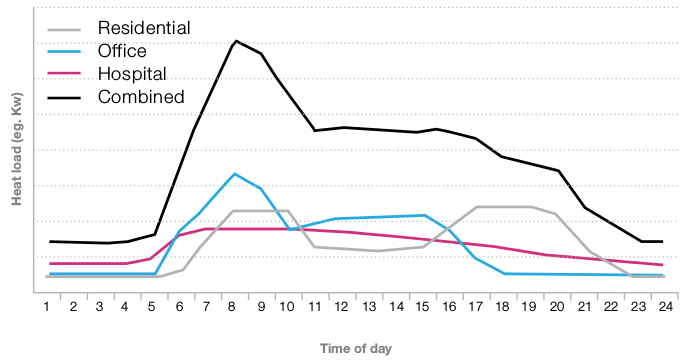
\includegraphics[width=0.7\linewidth]{mixLoad.png}
  \caption[Mixing Load Graph]{Mixing Load of Different Building
    Type~\cite{decentralHeatMap2011}}
  \label{fig:mixLoad}
\end{figure}

\subsection{Aggregation of Peak Value Becomes Tricky for Data with
  Time Variation}
One common mistake for sizing a district thermal energy system is to
add up the peak demand of each terminal users. Since the peak demand
of individual buildings do not occur at the same time, the end result
of summing up the peak demand at each end point exceeds the actual
total demand peak of the community, hence with this approach, the
whole district system becomes excessively over-sized, which reduces
the whole system efficiency. A Dynamic Energy Map can reveal the
problem of such approaches by directly providing the aggregated
thermal energy demand for the community and for single buildings or
building sectors. It allows a side by side comparison of single
building demand and aggregated demand and eliminates the
misunderstanding of the demand aggregation. With the direct
information of aggregated thermal energy demand, it also assists
actually sizing a district thermal energy system.